% acmsmall-sample.tex, dated 24th May 2012
% This is a sample file for ACM small trim journals
% Users can also go through the FAQs available on the journal's submission webpage.
%
% Steps to compile: latex, bibtex, latex latex
%
% For tracking purposes => this is v1.3 - May 2012
\documentclass{acmlarge-edm}

% Metadata Information
\acmVolume{1}
\acmNumber{2}
\acmArticle{3}
\acmYear{2012}
\acmMonth{5}  % can also put in literal name

\usepackage{graphics}

%
%  Cool LaTeX resource:
%   http://en.wikibooks.org/wiki/LaTeX

\title{Properties of the Bayesian Knowledge Tracing Model}
\author{BRETT VAN DE SANDE
\affil{Arizona State University\\bvds@asu.edu}}


\begin{abstract}
Bayesian Knowledge Tracing is used very widely to
model student learning.  It comes in two different forms:
The first form is the Bayesian Knowledge Tracing {\em hidden Markov model} 
which predicts the probability of correct application of a skill 
as a function of the number of opportunities and the model parameters.  
%This model can be fit to student prerformance data to determine model
%parameters.  
We present an analytical solution to this model and show that
it is, in fact, a function of three parameters and has the 
functional form of an exponential.
The second form is the Knowledge Tracing {\em algorithm}
which uses student performance at each opportunity to apply
a skill to update the conditional probability that the 
student has learned that skill.
We use a fixed point analysis to study solutions of this 
model and find a range of parameters where it has
the desired behavior.

\end{abstract}

\keywords{Bayesian Knowledge Tracing, student modelling, hidden Markov
model}

\begin{document}

\bibliographystyle{acmlarge}

\begin{bottomstuff}
Funding for this research was provided by the Pittsburgh Science of
Learning Center which is funded by the National Science Foundation
award No. SBE-0836012.
\end{bottomstuff}

\maketitle

%
%  Had idea to look at extensions to BKT where the analytic solution
%  is  not feasible but use variation of parameters to find any
%  "identifiability problem" (degeneracies).  However, the two that I
%  know about, Lee and  Brunskill and Baker's models do not have any 
%  degeneracies.   Probably not worth the effort, since a random, very 
%  complicated model, in general, will not have any degeneracies.
%


\section{Introduction}

Since its introduction by Corbett and 
Anderson~\citeyear{corbett_knowledge_1995}, 
Bayesian Knowledge Tracing (BKT) has been widely applied
to studies of student learning and to various tutor systems.  
In addition, BKT often serves as the starting
%
%   Need examples of BKT-based models, only look at examples
%   where Identifiability Problem exists.
%
point for more complicated models of learning, for 
example~\cite{baker_improving_2008,lee_impact_2012}.
%  BKT comes in two flavors:  regular and unsweetened. 
Researchers have applied BKT in two distinct ways:  
The {\em Hidden Markov Model} (HMM) form and the 
{\em Knowledge Tracing Algorithm} form.
The purpose of this paper is to investigate solutions of both
forms of the BKT model.

The HMM form~\cite{beck_identifiability:_2007} of BKT 
predicts the probability of that a student will 
correctly apply a skill when they have an opportunity to apply it.
%
% In the original Corbett and Anderson paper, they do not say
% how they fix the model parameters.  baker_ensembling_2011 and
% chang_bayes_2006  describes it as "curve fitting" and Baker private
% email to me says they used SSR. 
%
% Also "The Sum is Greater than the Parts: Ensembling Student
% Knowledge Models in ASSISTments" by Gowda et al. for KDD 2011
% Workshop uses RSS, but I can't get bibliographic info.
%
% chang_bayes_2006 also uses "curve fitting"
%
Typically, this model is fit to student performance data 
using either a residual sum of squares (RSS)
test (sometimes described as ``curve fitting'')
\cite{corbett_knowledge_1995} or a Maximum Likelihood
test~\cite{pardos_navigating_2010}, with several studies comparing the two
approaches~\cite{baker_ensembling_2011,chang_bayes_2006,pardos_ensembling_2011,pardos_sum_2012}.  The fit is then used to fix the model parameters.
%While using this model,  number of authors have noted have noted the 
%existence of what is called the ``Identifiability Problem'' 
%\cite{beck_identifiability:_2007}.    
%That is, there are certain combinations of the model 
%parameters that produce identical models.   
A typical HMM must be solved numerically to find its functional form.
However, this form of the model is simple enough that it can be 
solved analytically, which we will do here.  We will see that the model, 
in functional form, is an exponential.  Moreover, we will see that 
it is, in fact, a three parameter model.  As we shall see, 
this explains the ``Identifiability Problem'' first noted by 
Beck and Chang~\citeyear{beck_identifiability:_2007}.

%There are several reasons why a HMM is a good representation.  First,
%the parameters of the HMM are often thought to have some physical
%significance.  In BKT, for instance, $P(L_j)$ is the probability that the
%student knows the skill at a certain point of time:  it is a simple
%mental model of the student.  Thus, a distinction can be made between
%the student's mental state and their actual behavior (whether they
%can apply the skill correctly).   In contrast, a more behaviorist
%approach would eschew $P(L_j)$ in favor of a model of actual behavior.

Knowledge Tracing Algorithm form~\cite{corbett_knowledge_1995} 
of BKT is used to 
determine in real time whether a student has learned a skill.
The probability that the student has learned a skill is 
updated by student performance at each opportunity to apply
that skill.  The model has four parameters which must be 
supplied externally.  Although, this form of BKT is too complicated
to solve analytically, we will use a fixed point analysis to
study the behavior of its solutions.  This leads to constraints on 
possible model parameters.

\section{Hidden Markov Model form}

The Bayesian Knowledge Trading model~\cite{corbett_knowledge_1995} 
has four parameters:
%
\begin{itemize}
   \item $P(L_0)$ is the initial probability of knowing a skill.
   \item $P(G)$ is probability of guessing correctly, if the student        
         doesn't know the skill.
   \item $P(S)$ is probability of slips, if student does know the skill.
   \item $P(T)$ is probability of learning the skill if the student 
         does not know the skill.  Note that $P(T)$ is assumed to 
         be constant over steps.
\end{itemize}
%
Let $P(L_j)$ be the probability that the student knows the skill at 
step $j$. According to the model,  $P(L_j)$ can
be determined from the previous opportunity:
%
\begin{equation}
          P(L_j) = P(L_{j-1}) + P(T)\left(1-P(L_{j-1})\right)  \; . 
        \label{recurse}
\end{equation}
%
In this model, the probability that the student actually gets
opportunity $j$ correct is:
%
\begin{equation}
        P(C_j) = P(G)\left(1-P(L_j)\right) + \left(1-P(S)\right) P(L_j) \; . 
         \label{pnc}
\end{equation}
%
%(Unlike the four model parameters above, there isn't a consistent
%notation for $P(C_j)$ in the literature.)  
Eqns.~(\ref{recurse}) and (\ref{pnc}) define a hidden Markov model, 
where $P(L_j)$ is the ``hidden'' variable.

\begin{figure}
\centering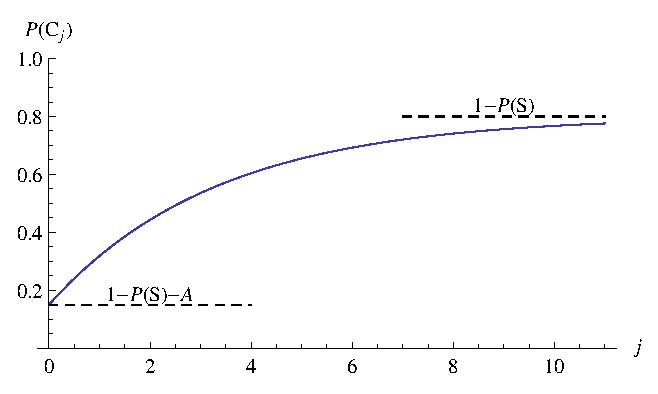
\includegraphics{exponential.eps}
\caption{Solution of the hidden Markov model form of BKT.
          $P(C_j)$ is the probability of  the student getting step $j$
          correct.  Note that the solution has the functional form of
          an exponential; see Eqn.~(\ref{solnn}).}
\label{bktgraph}
\end{figure}

This model can be  solved exactly.  First, we rewrite (\ref{recurse}) 
in a more suggestive form:
%
\begin{equation}
        1-P(L_j) = \left(1-P(T)\right) \left(1-P(L_{j-1})\right) \; .
\end{equation}
%
One can show that this recursion relation has solutions of the form:
%
\begin{equation}
            1-P(L_j) = \left(1-P(T)\right)^j\left(1-P(L_0)\right) \; .
	    \label{sol}
\end{equation}
%
%
Substituting (\ref{sol}) into (\ref{pnc}), we get:
%
\begin{equation}
        P(C_j) = 1-P(S) -\left(1-P(S)-P(G)\right) \left(1-P(L_0)\right)
                   \left(1-P(T)\right)^j \; . \label{pncsoln}
\end{equation}
%
Note that the form of $P(C_j)$, as a function of $j$, 
depends on only {\em three} parameters:  $P(S)$, $P(T)$, and 
$\left(1-P(S)-P(G)\right) \left(1-P(L_0)\right)$.
If we define
%
\begin{equation} 
          A=\left(1-P(S)-P(G)\right) \left(1-P(L_0)\right)  \label{aa}
\end{equation}
%
 and $\beta=-\log(1-P(T))$, then we can rewrite (\ref{pncsoln}) in 
a clearer form:
%
\begin{equation}
         P(C_j) = 1-P(S) -A e^{-\beta j} \, . \label{solnn}
\end{equation}
%
Thus, $P(C_j)$ is an exponential; see Fig.~\ref{bktgraph}.


\section{Identifiability and Parameter Constraints}

\begin{figure}
\centering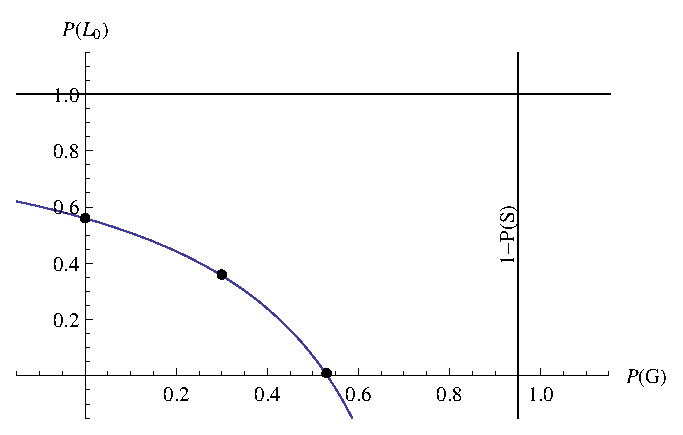
\includegraphics{table1.eps}
\caption{The relation between the guess rate $P(G)$ and the initial
  learning rate $P(L_0)$ for the hidden
  Markov model form of BKT.  All points along the curve correspond
  to identical models.
  The curve is a plot of solutions to Eqn.~(\ref{aa}), with $P(S)=0.05$ and $A=0.416$.
  The three points are the three parameter sets listed in Table~1 of
  \cite{beck_identifiability:_2007}.
}
 \label{table1}
\end{figure}

The fact that the Markov model is a function of three parameters
was first noticed by Beck and Chang~\citeyear{beck_identifiability:_2007} 
where they call it the ``Identifiability Problem.''   In their paper, 
they noted that multiple combinations of $P(G)$ and $P(L_0)$ give
exactly the same error rate $P(C_j)$, but do not explain the origin of 
these degenerate solutions.  An example showing the relation
between $P(G)$ and $P(L_0)$ for a given model is shown in Fig.~\ref{table1}.
Thus, we can see that Eqn.~(\ref{aa}) provides an explanation
of the Identifiability problem.

For the model to make sense, all probabilities should lie between 
zero and one.  In particular, $0\le P(L_0)\le 1$ and $0\le P(G) \le 1$.
If we further demand that learning is positive (which may or may not be
empirically justified), then we have the constraint $A>0$ or $P(G)+P(S)<1$.  
These constraints on $P(L_0)$ and $P(G)$ correspond to the rectangular
region shown in Fig.~\ref{table1}. 
In terms of $A$, valid values of $P(G)$ and $P(L_0)$ occur when
$0<A<1-P(S)$; for negative learning, meaningful values occur when
$-P(S)<A<0$.  This sets the range of physically meaningful values of
$A$ when fitting to student data.

Note that it is reasonable for the HMM form of the model to find
negative learning when fitting to student data.  If the student does
well on the first opportunities to apply a skill and then poorly on latter
opportunities, then the best fit to the student data will be a
decreasing function, which corresponds to $A<0$.  However,
we will see that such model parameters are problematic when
used as input for the Knowledge Tracing Algorithm.

\section{Bayesian Knowledge Tracing Algorithm}

\begin{figure}
\centering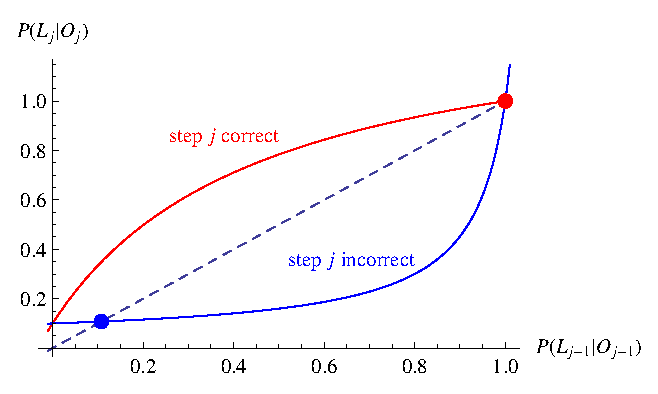
\includegraphics{p-recursion.eps}
\caption{
  Plot of the recursion relations for the Knowledge Tracing Algorithm, 
  Eqns.~(\ref{correct}) and (\ref{incorrect}).
  The stable fixed point for each equation is marked
  by a dot.  Since the ``step $j$ correct'' curve is above the
  dashed line, Eqn.~(\ref{correct}) causes $P(L_j|O_j)$ to converge to
  the fixed point at 1.  Likewise, since the ``step $j$ incorrect''
  curve is below the line, Eqn.~(\ref{incorrect}) causes $P(L_j|O_j)$
  to converge to the lower fixed point.
  Model parameters are $P(S)=0.05$, $P(G)=0.3$,  $P(T)=0.1$, and $P(L_0)=0.36$.
 }
 \label{p-recursion}
\end{figure}


%So far, we have discussed using BKT as a model which, when expressed
%in functional form, can be fitted to empirical data to obtain values
%for the three model parameters.  
In order to predict $P(L_j)$ for an individual student in real time,
the Knowledge Tracing Algorithm~\cite{corbett_knowledge_1995} may be employed.
In this case, we find $P(L_j|O_j)$,  the probability that the student has 
learned a skill just after completing step $j$ given student
performance $O_j$ on previous steps, where $O_j=\left\{o_1,\ldots,o_j\right\}$ is the student performance
on the first $j$ opportunities and $o_i$ can be either correct or
incorrect.  This conditional probability obeys the
recursion~\cite{baker_more_2008}: 
%
\begin{eqnarray}
       P(L_{j-1}|O_j) &=&
       \frac{P(L_{j-1}|O_{j-1})\left(1-P(S)\right)}{P(L_{j-1}|O_{j-1})\left(1-P(S)\right)+
                                       \left[1-P(L_{j-1}|O_{j-1})\right]P(G)}
                                     \; , \;\; o_j=\mbox{correct}\\
        P(L_{j-1}|O_j) &=& 
              \frac{P(L_{j-1}|O_{j-1}) P(S)}
              {P(L_{j-1}|O_{j-1}) P(S)+ \left[1-P(L_{j-1}|O_{j-1})\right]\left(1-P(G)\right)}
                        \; , \;\; o_j=\mbox{incorrect}\\
       P(L_j|O_j) &=& P\left(L_{j-1}|O_j\right)+
               \left[1-P(L_{j-1}|O_j)\right] P(T)
\end{eqnarray}
%
These equations can be combined to give:
%
\begin{eqnarray}
       P(L_j|O_j) &=&
       1-\frac{\left(1-P(T)\right)\left[1-P(L_{j-1}|O_{j-1})\right]P(G)}{P(G)+\left(1-P(S)-P(G)\right)
        P(L_{j-1}|O_{j-1})}  \;,\;\; o_j=\mbox{correct} \label{correct}\\
      P(L_j|O_j) &=& 1-\frac{\left(1-P(T)\right)\left[1-P(L_{j-1}|O_{j-1})\right]\left(1-P(G)\right)}
                                 {1-P(G)-\left(1-P(S)-P(G)\right) P(L_{j-1}|O_{j-1})}
                        \; ,\;\; o_j=\mbox{incorrect} \; . \label{incorrect}
\end{eqnarray}
%
%  corrupted
Their functional forms are plotted in Fig.~\ref{p-recursion}.  

While this recursion relation cannot be solved analytically, we can learn
much about its solutions by conducting a fixed point analysis. 
This is a technique that is covered in many differential equations textbooks; for
example, see \cite{blanchard_differential_2006}.  The the goal of this 
analysis is to determine the qualitative behavior of the sequence $P(L_j|O_j)$ as a
function of $j$.  If $P(L_j|O_j)>P(L_{j-1}|O_{j-1})$, then we know that $P(L_j|O_j)$
increases with $j$.  Likewise, if $P(L_j|O_j)<P(L_{j-1}|O_{j-1})$,
then we know that $P(L_j|O_j)$ decreases with $j$.  Thus, the case
$P(L_j|O_j)=P(L_{j-1}|O_{j-1})$, shown as the dashed line in Fig.~\ref{p-recursion}, 
serves as a boundary between increasing and decreasing solutions.
A {\em fixed point} is a value of $P(L_j|O_j)$ such that the recursion
relation obeys $P(L_j|O_j)=P(L_{j-1}|O_{j-1})$.  In the example at
hand, there are two kinds of fixed points:
\begin{description}
  \item[Stable fixed point] The sequence $P(L_j|O_j)$ moves toward the fixed point
    as $j$ increases;
  \item[Unstable fixed point] The sequence $P(L_j|O_j)$ moves away from the fixed as $j$ increases.
\end{description}

Let us apply these ideas to Eqns.~(\ref{correct}) and (\ref{incorrect}).
For Eqn.~(\ref{correct}), we find a stable fixed point at $1$ and 
an unstable fixed point at
%
\begin{equation}
    - \frac{P(G) P(T)}{1-P(G)-P(S)} \; .
      \label{correctfixedpoint}
\end{equation}
%
Similarly, Eqn.~(\ref{incorrect}) has an unstable fixed point at $1$
and a stable fixed point at
%
\begin{equation}
    \frac{\left(1-P(G)\right) P(T)}{1-P(G)-P(S)} \; . 
       \label{incorrectfixedpoint}
\end{equation}
%
The two stable fixed points are plotted as dots in Fig.~\ref{p-recursion}.


In order for $P(L_j|O_j)$ to remain in the interval $\left[0,1\right]$ 
for any starting value $P(L_0)\in \left[0,1\right]$ and any sequence of 
correct/incorrect steps $O_j$, 
we need the stable fixed point (\ref{incorrectfixedpoint})
to lie in the interval $\left[0,1\right]$ and the unstable fixed point 
(\ref{correctfixedpoint}) to remain negative.  This gives us the following
constraints on allowed values for the model parameters:
%
\begin{eqnarray}
        P(G)+P(S)&<& 1 \;, \label{littleconstraint}\\
        0 < P(T) &<& 1-\frac{P(S)}{1-P(G)}  \; .
        \label{bigconstraint}
\end{eqnarray}
%
If we instead choose parameters consistent with negative learning,
$P(S)+P(G)>1$, we find that the behavior of $P(L_j|O_j)$ becomes inverted: 
$P(L_j|O_j)$ decreases for correct steps and increases for incorrect steps.

Baker, Corbett, and Aleven~\citeyear{baker_more_2008} discuss the need
to choose model parameters such that the BKT algorithm behaves in a sensible
fashion.  In particular, they point out that correct actions by
the student should cause the estimate of their learning
$P(L_j|O_j)$ to increase.  They define models that do not have
this property to be ``empirically degenerate.''   Our constraint
(\ref{littleconstraint}) identifies precisely which models will be ``empirically
degenerate.''  Note that \cite{baker_more_2008} impose the somewhat
stronger constraints $P(S)<1/2$ and $P(G)<1/2$ on grounds that slip and
guess rates that are very large are simply nonsensical.

%For incorrect actions, the situation is
%more complicated since the model allows
%for the possibility that the student learns the skill during an incorrect
%step.  Thus, incorrect responses to not cause learning to converge
%to zero, but to the stable fixed point given by Eqn.~(\ref{incorrectfixedpoint}).
%Because of this, if $P(L_j|O_j)$ is below the stable fixed point, it
%will then increase with increasing $j$, even for incorrect

\begin{figure}
\centering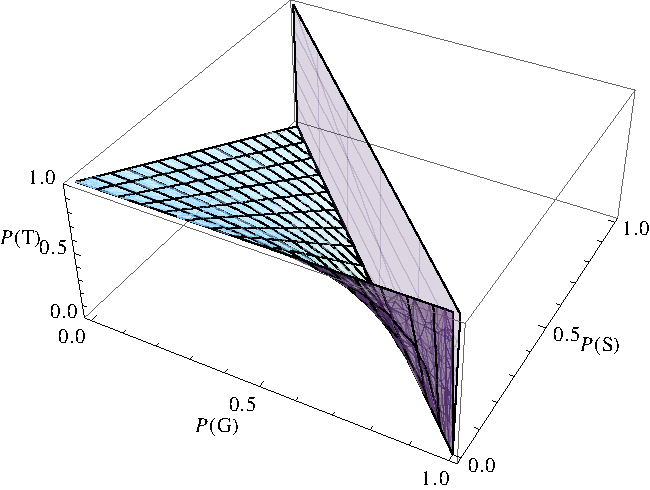
\includegraphics{region.pdf}
\caption{
  Plot of the constraint on the learning rate $P(T)$
  as a function of the  guess rate $P(G)$ and the
  slip rate $P(S)$ given by  Eqn.~(\ref{bigconstraint}).  Valid model parameter lie in the region 
  that is below this surface and above the $P(T)=0$ plane.  The
  vertical surface represents the other constraint $ P(G)+P(S)< 1 $,
  Eqn.~(\ref{littleconstraint}); valid model parameters lie to the left of this surface.
}
 \label{region}
\end{figure}


In terms of the parameter space, Eqn.~(\ref{bigconstraint})
provides a significant constraint on allowed values of model
parameters; see Fig.~\ref{region}.  In fact, it completely supersedes the
other constraint $P(G)+P(S)<1$.
It would be interesting to see how often this constraint is 
violated in real tutor systems, such as the 
Cognitive Tutors~\cite{ritter_cognitive_2007}, where the Knowledge
Tracing algorithm is used.

Finally, the ``Identifiability Problem'' for the Knowledge Tracing Algorithm
does not exist, so long as there are both correct and incorrect steps.
This fact can be seen by examining Eqns.~(\ref{correct}) and (\ref{incorrect})
where we see that $P(G)$ has a different functional form in
the numerator of each equation.  Thus, any redefinition of $1-P(L_j|O_j)$ 
cannot be compensated for by a redefinition
of other parameters in both  (\ref{correct}) and (\ref{incorrect}).
That is, all four model parameters independently affect the behavior
of the Knowledge Tracing Algorithm.


\section{Conclusion}


In conclusion, the hidden Markov model form of BKT, when expressed
in functional form, is an exponential function with three parameters.
Expressing the model in terms of three parameters should 
improve the speed and stability of any RSS or maximum likelihood 
fit to student data.  In that case, if $P(G)$ or
$P(L_0)$ is needed as output, then we suggest finding $A$ by
the fitting process,  fixing $P(G)$ or $P(L_0)$ by some 
external constraint, and using Eqn.~(\ref{aa}) to find the remaining
variable.
This would be an alternative to the Dirichlet 
priors~\cite{beck_identifiability:_2007} approach used by
some authors, but is much easier to implement, and does not
modify the model itself.  Typically, Dirichlet priors are applied
to all four model parameters, which is functionally equivalent to modifying the model itself.

Our other result is that the functional form of the Markov model 
corresponds to an exponential, rather than a power law.  
Heathcote, Brown, and Mewhort~\citeyear{heathcote_power_2000}
argue that learning for individuals is better described by an
exponential while (as shown in earlier studies) learning averaged
over individuals is better described by a power law function.
However, this analysis was performed using mainly reaction time
(latency) for tasks that were already learned, while we are interested
in the initial acquisition of a skill.  A recent study that focused
on students learning physics skills found that student learning
was better explained by a power law function, even for individual 
students~\cite{chi_instructional_2011}.
Together, these results call into question the popular practice of 
fitting the Markov model form of BKT to student data. 
Perhaps a model that has power law behavior would work better?

Finally, we see that the Knowledge Tracing Algorithm does not suffer from
the Identifiability Problem:  all four model parameters
affect model behavior separately.  
We also see that, for the model to behave properly,  there are 
significant constraints on the allowed values of $P(S)$, $P(G)$, and $P(T)$
and that parameters consistent with negative learning are not allowed.
It would be interesting to apply to see how often these constraints are
violated in tutor systems that employ the Knowledge Tracing Algorithm.
Finally, the fixed point analysis that we conducted here could be
applied to more complicated models of learning, such 
as~\cite{baker_improving_2008,lee_impact_2012}.


\begin{acks}
I would like to thank Ken Koedinger, Michael Yudelson, and Tristan Nixon for
useful comments.
\end{acks}

\bibliography{education-modeling}

\end{document}